\chapter{Einführung}
Secure Multiparty Computation ein großes Forschungsfeld in der Kryptographie, in dem zwar schon in den 1980er Jahren die Forschung begann, das aber seit den 2000er Jahren mehr Aufmerksamkeit bekommt. \cite{Kogan2021}
In diesem Forschungsfeld werden Methoden erforscht, mit denen gemeinsam Funktionen von Eingabedaten berechnet werden können, ohne dass dabei die anderen teilnehmenden Parteien die Eingabedaten erhalten.\\
Nachdem die Forschungsergebnisse in den 80ern eher theoretisch waren, sind die neueren Forschungen eher praktisch. Denn durch mehrere Effekte wurden die Berechnungen erst in breiteren Anwendungsbereichen sinnvoll nutzbar. Einerseits wurden die berechnenden Computer stärker, beispielsweise hat sich die CPU Geschwindigkeit in PCs ungefähr verdoppelt. Das allein kann aber noch nicht die mehr als 60.000 fache Beschleunigung der Berechnungsgeschwindigkeit erklären. \cite{Kogan2021}
\begin{figure}[h]
\begin{center}
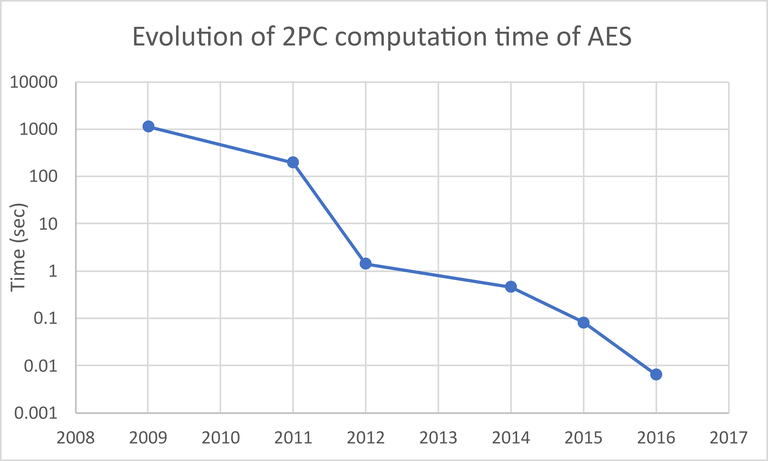
\includegraphics[width = 8cm]{comptime.png}
\caption{Die Veränderung der Berechnungzeit für secure computation}
\cite{Kogan2021}
\label{evolution_of_computation}

\end{center}

\end{figure}


Durch die Grafik \ref{evolution_of_computation} wird die sich immer weiter verbessernde Geschwindigkeit der secure computation Protokolle deutlich. Zur erleichterten Lesbarkeit zeigt die Grafik zwar nur die Berechnungszeiten für zwei Parteien, dennoch wird deutlich, dass sich durch die Forschung in diesem Bereich die Effizienz von secure computation Protokollen stark gesteigert hat.
Der größte Teil des Tempogewinns liegt also an den neuen oder verbesserten Protokollen, die entwickelt wurden.\\
Eine Funktion, die in vielen Bereichen interessant sein kann, ist die Schnittmenge der Eingabemengen der teilnehmenden Parteien. 2021 wurde \cite{Doettling2021} veröffentlicht. In diesem Paper wurde ein neues Protokoll vorgestellt, das genau diese Funktion erfüllt. Durch einen Effizienztest des Protokolls, kann nun festgestellt werden, ob dieses Protokoll funktioniert und effizient ist.

\section{Anwendungsbeispiel}
Der Browser Tor, den Menschen benutzen können, um in das sogenannte Darknet zu gelangen legt einen sehr großen Wert auf die Sicherheit der Nutzer. Das macht die Analyse bestimmter Statistiken sehr schwierig. Deshalb gibt es auch vom Anbieter selbst keine genauen Angaben über beispielsweise die Nutzerzahl, sondern nur Schätzungen. Um genauere Schätzungen über die Nutzerzahl zu ermöglichen, könnte man nun Daten von mehreren "Knoten" des Tor Browsers kombinieren. In diesem Fall möchte man gerne herausfinden, wie viele Überschneidungen es in den Daten der "Knoten" gibt, um Mehrfachzählungen zu vermeiden. Da viele Nutzer des Tor Browsers aber einen sehr großen Wert auf Sicherheit legen, möchte man natürlich tunlichst vermeiden, Daten von mehreren "Knoten" miteinander zu kombinieren, weil so möglicherweise Informationen gewonnen werden können, die geheim sein sollten.\\
Um zu garantieren, dass die Daten beispielsweise nur zur Ermittlung der Größe der Schnittmenge genutzt werden, können spezielle Protokolle genutzt werden, die die Daten nur verschlüsselt benutzen und nur ganz bestimmte  Analysen auf den verschlüsselten Daten erlauben. So können Statistiken über den Tor Browser erstellt werden, ohne dass die Gefahr besteht, dass Informationen der Nutzer zugänglich werden.

\section{Zielsetzung}
Das Ziel der Arbeit ist es, die Effizienz der im Paper \cite{Doettling2021} vorgestellten neuen Protokolle zu testen. Einerseits, um zu demonstrieren, dass die vorgestellten Protokolle und Funktionalitäten korrekt funktionieren. Andererseits, um die neuen Funktionalitäten und ?Verschnellerungen? allen zugänglich zu machen.\\
Um die Funktionalitäten wie im Paper \cite{Doettling2021} beschrieben zu implementieren, werden auch Implementierungen von anderen Veröffentlichungen benötigt (\cite{Schoenmakers} Beispielsweise für das secureRank Teilprotokoll). Da zu diesem Zeitpunkt noch keine derartigen Implementierungen veröffentlicht sind, kann auch nicht auf diese Zurückgegriffen werden. Um trotzdem zu demonstrieren, dass das im \cite{Doettling2021} vorgestellte Protokoll funktioniert und effizient ist, habe ich die Unterprotokolle, die auf solche externen Paper zurückgreifen auf unsichere Weise implementiert. Dadurch funktioniert das Protokoll, und die unsicheren Unterprotokolle können ohne viel Zeitaufwand durch sichere Implementierungen ersetzt werden, wenn die Funktionalitäten der anderen Veröffentlichungen implementiert sind.

